
            \begin{tabular}{lll}
    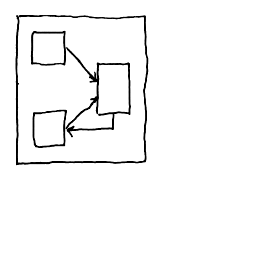
\includegraphics[width = 5cm]{../TikZ/drawings/expert-0.png}&
            
\includegraphics[width = 5cm]{../TikZ/drawings/expert-0-parses/0.png}&
    
        \begin{minipage}{10cm}
        \begin{verbatim}
line(6,2,6,3,
arrow = False,solid = True);
line(6,2,3,2,
arrow = True,solid = True);
reflect(y = 9){
line(3,7,5,5,
arrow = True,solid = True);
rectangle(1,1,3,3);
rectangle(5,3,7,6);
rectangle(0,0,8,9)
}
        \end{verbatim}
\end{minipage}

    \end{tabular}        
            \\

            \begin{tabular}{lll}
    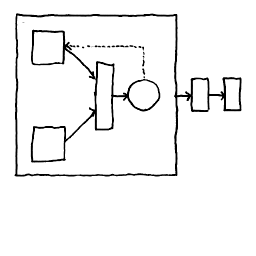
\includegraphics[width = 5cm]{../TikZ/drawings/expert-1.png}&
            
\includegraphics[width = 5cm]{../TikZ/drawings/expert-1-parses/0.png}&
    
        \begin{minipage}{10cm}
        \begin{verbatim}
for (i < 2){
line(8,8,3,8,
arrow = True,solid = False);
line(-2 * i + 12,5,-2 * i + 13,5,
arrow = True,solid = True);
line(6,5,7,5,
arrow = True,solid = True);
line(3,-6 * i + 8,5,-2 * i + 6,
arrow = True,solid = True);
rectangle(-2 * i + 13,4,-2 * i + 14,6);
rectangle(1,-6 * i + 7,3,-6 * i + 9)
};
circle(8,5);
rectangle(5,3,6,7);
rectangle(0,0,10,10);
line(8,6,8,8,
arrow = False,solid = False)
        \end{verbatim}
\end{minipage}

    \end{tabular}        
            \\

            \begin{tabular}{lll}
    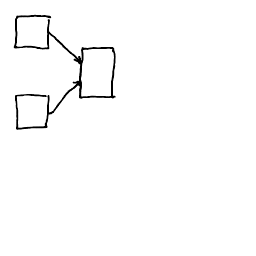
\includegraphics[width = 5cm]{../TikZ/drawings/expert-2.png}&
            
\includegraphics[width = 5cm]{../TikZ/drawings/expert-2-parses/0.png}&
    
        \begin{minipage}{10cm}
        \begin{verbatim}
reflect(y = 7){
line(2,6,4,4,
arrow = True,solid = True);
rectangle(0,0,2,2)
};
rectangle(4,2,6,5)
        \end{verbatim}
\end{minipage}

    \end{tabular}        
            \\

            \begin{tabular}{lll}
    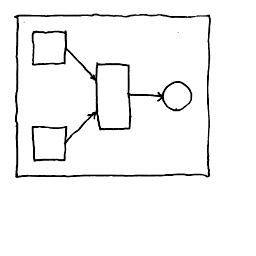
\includegraphics[width = 5cm]{../TikZ/drawings/expert-3.png}&
            
\includegraphics[width = 5cm]{../TikZ/drawings/expert-3-parses/0.png}&
    
        \begin{minipage}{10cm}
        \begin{verbatim}
line(7,5,9,5,
arrow = True,solid = True);
rectangle(5,3,7,7);
rectangle(0,0,12,10);
reflect(y = 10){
circle(10,5);
line(3,2,5,4,
arrow = True,solid = True);
rectangle(1,1,3,3)
}
        \end{verbatim}
\end{minipage}

    \end{tabular}        
            \\

            \begin{tabular}{lll}
    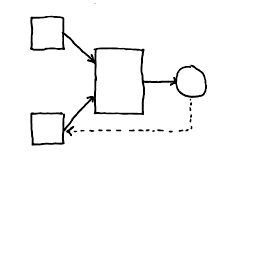
\includegraphics[width = 5cm]{../TikZ/drawings/expert-4.png}&
            
\includegraphics[width = 5cm]{../TikZ/drawings/expert-4-parses/0.png}&
    
        \begin{minipage}{10cm}
        \begin{verbatim}
line(10,1,2,1,
arrow = True,solid = False);
line(10,1,10,3,
arrow = False,solid = False);
line(7,4,9,4,
arrow = True,solid = True);
reflect(y = 8){
circle(10,4);
line(2,1,4,3,
arrow = True,solid = True);
rectangle(4,2,7,6);
rectangle(0,6,2,8)
}
        \end{verbatim}
\end{minipage}

    \end{tabular}        
            \\

            \begin{tabular}{lll}
    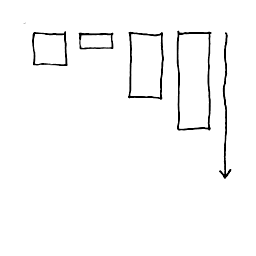
\includegraphics[width = 5cm]{../TikZ/drawings/expert-5.png}&
            
\includegraphics[width = 5cm]{../TikZ/drawings/expert-5-parses/0.png}&
    
        \begin{minipage}{10cm}
        \begin{verbatim}
line(12,9,12,0,
arrow = True,solid = True);
rectangle(9,3,11,9);
rectangle(6,5,8,9);
rectangle(0,7,2,9);
rectangle(3,8,5,9)
        \end{verbatim}
\end{minipage}

    \end{tabular}        
            \\

            \begin{tabular}{lll}
    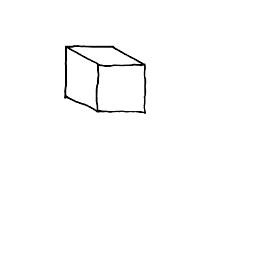
\includegraphics[width = 5cm]{../TikZ/drawings/expert-6.png}&
            
\includegraphics[width = 5cm]{../TikZ/drawings/expert-6-parses/0.png}&
    
        \begin{minipage}{10cm}
        \begin{verbatim}
for (i < 3){
for (j < (1*i + 1)){
if (j > 0){
line(3 * j + -3,3 * i + -2,3 * j + -1,3 * i + -3,
arrow = False,solid = True);
line(0,3 * j + -2,3 * j + -3,4,
arrow = False,solid = True)
}
rectangle(2,0,5,3)
}
}
        \end{verbatim}
\end{minipage}

    \end{tabular}        
            \\

            \begin{tabular}{lll}
    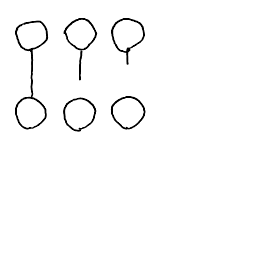
\includegraphics[width = 5cm]{../TikZ/drawings/expert-7.png}&
            
\includegraphics[width = 5cm]{../TikZ/drawings/expert-7-parses/0.png}&
    
        \begin{minipage}{10cm}
        \begin{verbatim}
for (i < 3){
circle(-3 * i + 7,1);
circle(-3 * i + 7,6);
line(-3 * i + 7,-1 * i + 4,-3 * i + 7,5,
arrow = False,solid = True)
}
        \end{verbatim}
\end{minipage}

    \end{tabular}        
            \\

            \begin{tabular}{lll}
    
\includegraphics[width = 5cm]{../TikZ/drawings/expert-8.png}&
            
\includegraphics[width = 5cm]{../TikZ/drawings/expert-8-parses/0.png}&
    
        \begin{minipage}{10cm}
        \begin{verbatim}
line(0,0,0,4,
arrow = False,solid = True)
        \end{verbatim}
\end{minipage}

    \end{tabular}        
            \\

            \begin{tabular}{lll}
    
\includegraphics[width = 5cm]{../TikZ/drawings/expert-9.png}&
            
\includegraphics[width = 5cm]{../TikZ/drawings/expert-9-parses/0.png}&
    
        \begin{minipage}{10cm}
        \begin{verbatim}
line(6,0,0,0,
arrow = True,solid = True)
        \end{verbatim}
\end{minipage}

    \end{tabular}        
            \\

            \begin{tabular}{lll}
    
\includegraphics[width = 5cm]{../TikZ/drawings/expert-10.png}&
            
\includegraphics[width = 5cm]{../TikZ/drawings/expert-10-parses/0.png}&
    
        \begin{minipage}{10cm}
        \begin{verbatim}
rectangle(0,0,3,4)
        \end{verbatim}
\end{minipage}

    \end{tabular}        
            \\

            \begin{tabular}{lll}
    
\includegraphics[width = 5cm]{../TikZ/drawings/expert-11.png}&
            
\includegraphics[width = 5cm]{../TikZ/drawings/expert-11-parses/0.png}&
    
        \begin{minipage}{10cm}
        \begin{verbatim}
circle(1,1)
        \end{verbatim}
\end{minipage}

    \end{tabular}        
            \\

            \begin{tabular}{lll}
    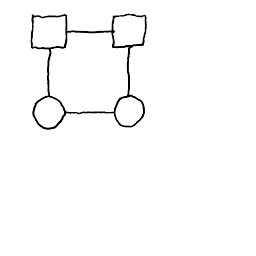
\includegraphics[width = 5cm]{../TikZ/drawings/expert-12.png}&
            
\includegraphics[width = 5cm]{../TikZ/drawings/expert-12-parses/0.png}&
    
        \begin{minipage}{10cm}
        \begin{verbatim}
reflect(x = 7){
circle(6,1);
line(6,2,6,5,
arrow = False,solid = True);
rectangle(5,5,7,7)
};
line(2,6,5,6,
arrow = False,solid = True);
line(2,1,5,1,
arrow = False,solid = True)
        \end{verbatim}
\end{minipage}

    \end{tabular}        
            \\

            \begin{tabular}{lll}
    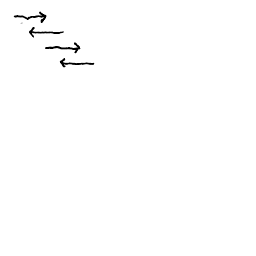
\includegraphics[width = 5cm]{../TikZ/drawings/expert-13.png}&
            
\includegraphics[width = 5cm]{../TikZ/drawings/expert-13-parses/0.png}&
    
        \begin{minipage}{10cm}
        \begin{verbatim}
line(3,2,1,2,
arrow = True,solid = True);
line(0,3,2,3,
arrow = True,solid = True);
line(5,0,3,0,
arrow = True,solid = True);
line(2,1,4,1,
arrow = True,solid = True)
        \end{verbatim}
\end{minipage}

    \end{tabular}        
            \\

            \begin{tabular}{lll}
    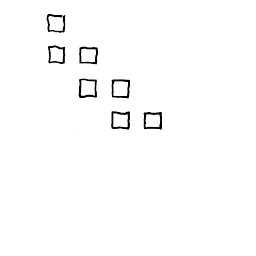
\includegraphics[width = 5cm]{../TikZ/drawings/expert-14.png}&
            
\includegraphics[width = 5cm]{../TikZ/drawings/expert-14-parses/0.png}&
    
        \begin{minipage}{10cm}
        \begin{verbatim}
rectangle(6,0,7,1);
for (i < 3){
rectangle(-2 * i + 4,2 * i + 2,-2 * i + 5,2 * i + 3);
rectangle(-2 * i + 4,2 * i,-2 * i + 5,2 * i + 1)
}
        \end{verbatim}
\end{minipage}

    \end{tabular}        
            \\

            \begin{tabular}{lll}
    
\includegraphics[width = 5cm]{../TikZ/drawings/expert-15.png}&
            
\includegraphics[width = 5cm]{../TikZ/drawings/expert-15-parses/0.png}&
    
        \begin{minipage}{10cm}
        \begin{verbatim}
line(3,0,5,0,
arrow = False,solid = True);
line(1,2,3,2,
arrow = False,solid = True);
line(0,3,2,3,
arrow = False,solid = False);
line(2,1,4,1,
arrow = False,solid = False)
        \end{verbatim}
\end{minipage}

    \end{tabular}        
            \\

            \begin{tabular}{lll}
    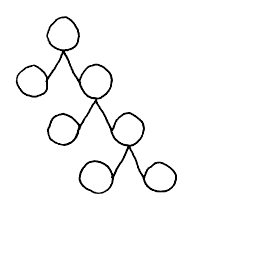
\includegraphics[width = 5cm]{../TikZ/drawings/expert-16.png}&
            
\includegraphics[width = 5cm]{../TikZ/drawings/expert-16-parses/0.png}&
    
        \begin{minipage}{10cm}
        \begin{verbatim}
circle(9,1);
for (i < 3){
circle(-2 * i + 7,3 * i + 4);
circle(-2 * i + 5,3 * i + 1);
line(-2 * i + 6,3 * i + 1,-2 * i + 7,3 * i + 3,
arrow = False,solid = True);
line(-2 * i + 7,3 * i + 3,-2 * i + 8,3 * i + 1,
arrow = False,solid = True)
}
        \end{verbatim}
\end{minipage}

    \end{tabular}        
            \\

            \begin{tabular}{lll}
    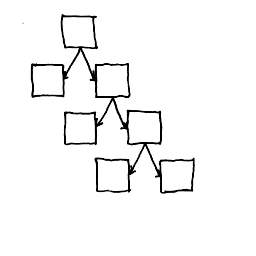
\includegraphics[width = 5cm]{../TikZ/drawings/expert-17.png}&
            
\includegraphics[width = 5cm]{../TikZ/drawings/expert-17-parses/0.png}&
    
        \begin{minipage}{10cm}
        \begin{verbatim}
for (i < 3){
line(2 * i + 3,-3 * i + 9,2 * i + 2,-3 * i + 7,
arrow = True,solid = True);
line(2 * i + 3,-3 * i + 9,2 * i + 4,-3 * i + 7,
arrow = True,solid = True);
rectangle(2 * i + 2,-3 * i + 9,2 * i + 4,-3 * i + 11);
rectangle(2 * i,-3 * i + 6,2 * i + 2,-3 * i + 8)
};
rectangle(8,0,10,2)
        \end{verbatim}
\end{minipage}

    \end{tabular}        
            \\

            \begin{tabular}{lll}
    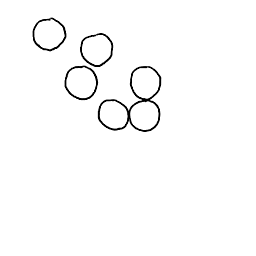
\includegraphics[width = 5cm]{../TikZ/drawings/expert-18.png}&
            
\includegraphics[width = 5cm]{../TikZ/drawings/expert-18-parses/0.png}&
    
        \begin{minipage}{10cm}
        \begin{verbatim}
for (i < 2){
circle(2 * i + 1,-3 * i + 6);
circle(-3 * i + 7,2 * i + 3);
circle(2 * i + 5,1)
}
        \end{verbatim}
\end{minipage}

    \end{tabular}        
            \\

            \begin{tabular}{lll}
    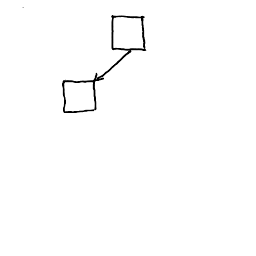
\includegraphics[width = 5cm]{../TikZ/drawings/expert-19.png}&
            
\includegraphics[width = 5cm]{../TikZ/drawings/expert-19-parses/0.png}&
    
        \begin{minipage}{10cm}
        \begin{verbatim}
line(4,4,2,2,
arrow = True,solid = True);
rectangle(0,0,2,2);
rectangle(3,4,5,6)
        \end{verbatim}
\end{minipage}

    \end{tabular}        
            \\

            \begin{tabular}{lll}
    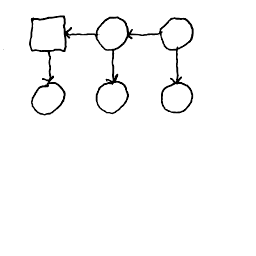
\includegraphics[width = 5cm]{../TikZ/drawings/expert-20.png}&
            
\includegraphics[width = 5cm]{../TikZ/drawings/expert-20-parses/0.png}&
    
        \begin{minipage}{10cm}
        \begin{verbatim}
for (i < 3){
line(-4 * i + 9,4,-4 * i + 9,2,
arrow = True,solid = True);
for (j < (1*i + 2)){
if (j > 0){
circle(-4 * j + 13,-4 * i + 9);
line(-4 * i + 12,5,-4 * i + 10,5,
arrow = True,solid = True)
}
rectangle(0,4,2,6)
}
}
        \end{verbatim}
\end{minipage}

    \end{tabular}        
            \\

            \begin{tabular}{lll}
    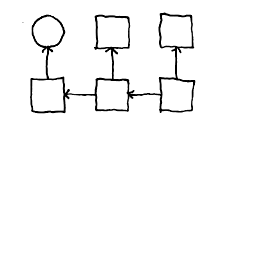
\includegraphics[width = 5cm]{../TikZ/drawings/expert-21.png}&
            
\includegraphics[width = 5cm]{../TikZ/drawings/expert-21-parses/0.png}&
    
        \begin{minipage}{10cm}
        \begin{verbatim}
circle(1,5);
line(4,1,2,1,
arrow = True,solid = True);
line(8,1,6,1,
arrow = True,solid = True);
for (i < 3){
line(4 * i + 1,2,4 * i + 1,4,
arrow = True,solid = True);
rectangle(4,4,6,6);
rectangle(4 * i,0,4 * i + 2,2)
};
rectangle(8,4,10,6)
        \end{verbatim}
\end{minipage}

    \end{tabular}        
            \\

            \begin{tabular}{lll}
    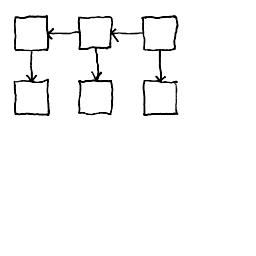
\includegraphics[width = 5cm]{../TikZ/drawings/expert-22.png}&
            
\includegraphics[width = 5cm]{../TikZ/drawings/expert-22-parses/0.png}&
    
        \begin{minipage}{10cm}
        \begin{verbatim}
for (i < 3){
line(4 * i + 1,4,4 * i + 1,2,
arrow = True,solid = True);
for (j < 2){
line(4 * j + 4,5,4 * j + 2,5,
arrow = True,solid = True);
rectangle(4 * i,-4 * j + 4,4 * i + 2,-4 * j + 6)
}
}
        \end{verbatim}
\end{minipage}

    \end{tabular}        
            \\

            \begin{tabular}{lll}
    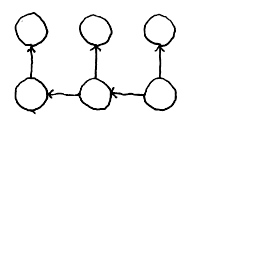
\includegraphics[width = 5cm]{../TikZ/drawings/expert-23.png}&
            
\includegraphics[width = 5cm]{../TikZ/drawings/expert-23-parses/0.png}&
    
        \begin{minipage}{10cm}
        \begin{verbatim}
for (i < 3){
line(4 * i + 1,2,4 * i + 1,4,
arrow = True,solid = True);
for (j < 2){
circle(4 * i + 1,4 * j + 1);
line(4 * j + 4,1,4 * j + 2,1,
arrow = True,solid = True)
}
}
        \end{verbatim}
\end{minipage}

    \end{tabular}        
            \\

            \begin{tabular}{lll}
    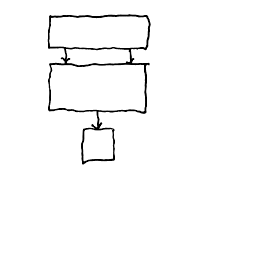
\includegraphics[width = 5cm]{../TikZ/drawings/expert-24.png}&
            
\includegraphics[width = 5cm]{../TikZ/drawings/expert-24-parses/0.png}&
    
        \begin{minipage}{10cm}
        \begin{verbatim}
line(5,7,5,6,
arrow = True,solid = True);
line(3,3,3,2,
arrow = True,solid = True);
line(1,7,1,6,
arrow = True,solid = True);
rectangle(0,3,6,6);
rectangle(2,0,4,2);
rectangle(0,7,6,9)
        \end{verbatim}
\end{minipage}

    \end{tabular}        
            \\

            \begin{tabular}{lll}
    \includegraphics[width = 5cm]{../TikZ/drawings/expert-25.png}&
            \includegraphics[width = 5cm]{../TikZ/drawings/expert-25-parses/0.png}&
    
        \begin{minipage}{10cm}
        \begin{verbatim}
line(6,1,5,1,
arrow = True,solid = True);
for (i < 3){
line(3,1,2,1,
arrow = True,solid = True);
rectangle(3 * i,0,3 * i + 2,2)
}
        \end{verbatim}
\end{minipage}

    \end{tabular}        
            \\

            \begin{tabular}{lll}
    \includegraphics[width = 5cm]{../TikZ/drawings/expert-26.png}&
            \includegraphics[width = 5cm]{../TikZ/drawings/expert-26-parses/0.png}&
    
        \begin{minipage}{10cm}
        \begin{verbatim}
for (i < 3){
circle(1,-4 * i + 9)
};
line(1,4,1,2,
arrow = True,solid = True);
line(1,8,1,6,
arrow = True,solid = True)
        \end{verbatim}
\end{minipage}

    \end{tabular}        
            \\

            \begin{tabular}{lll}
    \includegraphics[width = 5cm]{../TikZ/drawings/expert-27.png}&
            \includegraphics[width = 5cm]{../TikZ/drawings/expert-27-parses/0.png}&
    
        \begin{minipage}{10cm}
        \begin{verbatim}
reflect(y = 2){
line(0,1,1,2,
arrow = False,solid = True);
line(1,0,2,1,
arrow = False,solid = True)
}
        \end{verbatim}
\end{minipage}

    \end{tabular}        
            \\

            \begin{tabular}{lll}
    \includegraphics[width = 5cm]{../TikZ/drawings/expert-28.png}&
            \includegraphics[width = 5cm]{../TikZ/drawings/expert-28-parses/0.png}&
    
        \begin{minipage}{10cm}
        \begin{verbatim}
line(0,0,0,2,
arrow = False,solid = True);
line(0,2,2,2,
arrow = False,solid = True)
        \end{verbatim}
\end{minipage}

    \end{tabular}        
            \\

            \begin{tabular}{lll}
    \includegraphics[width = 5cm]{../TikZ/drawings/expert-29.png}&
            \includegraphics[width = 5cm]{../TikZ/drawings/expert-29-parses/0.png}&
    
        \begin{minipage}{10cm}
        \begin{verbatim}
for (i < 3){
line(1 * i,-2 * i + 4,1 * i,-1 * i + 6,
arrow = False,solid = True);
line(1 * i,-1 * i + 6,2 * i + 2,-1 * i + 6,
arrow = False,solid = True)
}
        \end{verbatim}
\end{minipage}

    \end{tabular}        
            \\

            \begin{tabular}{lll}
    \includegraphics[width = 5cm]{../TikZ/drawings/expert-30.png}&
            \includegraphics[width = 5cm]{../TikZ/drawings/expert-30-parses/0.png}&
    
        \begin{minipage}{10cm}
        \begin{verbatim}
circle(5,2);
circle(5,4);
rectangle(4,1,6,5);
reflect(y = 5){
circle(1,4);
rectangle(0,3,2,5)
}
        \end{verbatim}
\end{minipage}

    \end{tabular}        
            \\

            \begin{tabular}{lll}
    \includegraphics[width = 5cm]{../TikZ/drawings/expert-31.png}&
            \includegraphics[width = 5cm]{../TikZ/drawings/expert-31-parses/0.png}&
    
        \begin{minipage}{10cm}
        \begin{verbatim}
for (i < 3){
for (j < (1*i + 1)){
circle(3 * i + 1,-2 * j + 5)
};
rectangle(3 * i,-2 * i + 4,3 * i + 2,6)
}
        \end{verbatim}
\end{minipage}

    \end{tabular}        
            \\

            \begin{tabular}{lll}
    \includegraphics[width = 5cm]{../TikZ/drawings/expert-32.png}&
            \includegraphics[width = 5cm]{../TikZ/drawings/expert-32-parses/0.png}&
    
        \begin{minipage}{10cm}
        \begin{verbatim}
circle(5,5);
line(2,5,4,5,
arrow = False,solid = True);
rectangle(0,0,5,3);
rectangle(0,4,2,6)
        \end{verbatim}
\end{minipage}

    \end{tabular}        
            \\

            \begin{tabular}{lll}
    \includegraphics[width = 5cm]{../TikZ/drawings/expert-33.png}&
            \includegraphics[width = 5cm]{../TikZ/drawings/expert-33-parses/0.png}&
    
        \begin{minipage}{10cm}
        \begin{verbatim}
line(0,0,0,3,
arrow = False,solid = True);
line(6,0,6,3,
arrow = False,solid = True);
line(0,3,6,3,
arrow = False,solid = False);
line(0,0,6,0,
arrow = False,solid = False)
        \end{verbatim}
\end{minipage}

    \end{tabular}        
            \\

            \begin{tabular}{lll}
    \includegraphics[width = 5cm]{../TikZ/drawings/expert-34.png}&
            \includegraphics[width = 5cm]{../TikZ/drawings/expert-34-parses/0.png}&
    
        \begin{minipage}{10cm}
        \begin{verbatim}
for (i < 2){
line(2 * i,-2 * i + 5,2,5,
arrow = False,solid = True);
line(1,2,2 * i + 1,-2 * i + 4,
arrow = False,solid = True);
line(2 * i + 3,-2 * i + 3,5,3,
arrow = False,solid = True);
line(4,0,2 * i + 4,-2 * i + 2,
arrow = False,solid = True)
}
        \end{verbatim}
\end{minipage}

    \end{tabular}        
            \\

            \begin{tabular}{lll}
    \includegraphics[width = 5cm]{../TikZ/drawings/expert-35.png}&
            \includegraphics[width = 5cm]{../TikZ/drawings/expert-35-parses/0.png}&
    
        \begin{minipage}{10cm}
        \begin{verbatim}
circle(6,1);
circle(1,1);
circle(1,6);
line(2,6,6,2,
arrow = True,solid = True);
line(1,5,1,2,
arrow = True,solid = True)
        \end{verbatim}
\end{minipage}

    \end{tabular}        
            \\

            \begin{tabular}{lll}
    \includegraphics[width = 5cm]{../TikZ/drawings/expert-36.png}&
            \includegraphics[width = 5cm]{../TikZ/drawings/expert-36-parses/0.png}&
    
        \begin{minipage}{10cm}
        \begin{verbatim}
rectangle(5,5,9,9);
rectangle(0,0,4,4);
for (i < 2){
rectangle(1 * i + 7,-2 * i + 2,9,-3 * i + 4);
rectangle(0,-3 * i + 8,1 * i + 1,-2 * i + 9)
}
        \end{verbatim}
\end{minipage}

    \end{tabular}        
            \\

            \begin{tabular}{lll}
    \includegraphics[width = 5cm]{../TikZ/drawings/expert-37.png}&
            \includegraphics[width = 5cm]{../TikZ/drawings/expert-37-parses/0.png}&
    
        \begin{minipage}{10cm}
        \begin{verbatim}
circle(1,8);
line(5,2,5,5,
arrow = False,solid = True);
line(1,7,3,5,
arrow = False,solid = True);
rectangle(4,0,6,2);
rectangle(0,5,6,9)
        \end{verbatim}
\end{minipage}

    \end{tabular}        
            \\

            \begin{tabular}{lll}
    \includegraphics[width = 5cm]{../TikZ/drawings/expert-38.png}&
            \includegraphics[width = 5cm]{../TikZ/drawings/expert-38-parses/0.png}&
    
        \begin{minipage}{10cm}
        \begin{verbatim}
for (i < 3){
for (j < 3){
if (j > 0){
line(3 * j + -1,3 * i + 1,3 * j,3 * i + 1,
arrow = False,solid = True);
line(3 * i + 1,3 * j + -1,3 * i + 1,3 * j,
arrow = False,solid = True)
}
circle(3 * i + 1,3 * j + 1)
}
}
        \end{verbatim}
\end{minipage}

    \end{tabular}        
            \\

            \begin{tabular}{lll}
    \includegraphics[width = 5cm]{../TikZ/drawings/expert-39.png}&
            \includegraphics[width = 5cm]{../TikZ/drawings/expert-39-parses/0.png}&
    
        \begin{minipage}{10cm}
        \begin{verbatim}
for (i < 3){
for (j < 3){
if (j > 0){
line(3 * i + 1,3 * j + -1,3 * i + 1,3 * j,
arrow = False,solid = True);
line(3 * j + -1,3 * i + 1,3 * j,3 * i + 1,
arrow = False,solid = True)
}
rectangle(3 * i,3 * j,3 * i + 2,3 * j + 2)
}
}
        \end{verbatim}
\end{minipage}

    \end{tabular}        
            \\

            \begin{tabular}{lll}
    \includegraphics[width = 5cm]{../TikZ/drawings/expert-40.png}&
            \includegraphics[width = 5cm]{../TikZ/drawings/expert-40-parses/0.png}&
    
        \begin{minipage}{10cm}
        \begin{verbatim}
for (i < 3){
circle(-3 * i + 7,1)
}
        \end{verbatim}
\end{minipage}

    \end{tabular}        
            \\

            \begin{tabular}{lll}
    \includegraphics[width = 5cm]{../TikZ/drawings/expert-41.png}&
            \includegraphics[width = 5cm]{../TikZ/drawings/expert-41-parses/0.png}&
    
        \begin{minipage}{10cm}
        \begin{verbatim}
for (i < 3){
rectangle(-2 * i + 4,0,-2 * i + 5,6)
}
        \end{verbatim}
\end{minipage}

    \end{tabular}        
            \\

            \begin{tabular}{lll}
    \includegraphics[width = 5cm]{../TikZ/drawings/expert-42.png}&
            \includegraphics[width = 5cm]{../TikZ/drawings/expert-42-parses/0.png}&
    
        \begin{minipage}{10cm}
        \begin{verbatim}
line(4,0,4,1,
arrow = False,solid = False);
line(0,0,0,5,
arrow = False,solid = False);
line(4,1,4,5,
arrow = False,solid = False)
        \end{verbatim}
\end{minipage}

    \end{tabular}        
            \\

            \begin{tabular}{lll}
    \includegraphics[width = 5cm]{../TikZ/drawings/expert-43.png}&
            \includegraphics[width = 5cm]{../TikZ/drawings/expert-43-parses/0.png}&
    
        \begin{minipage}{10cm}
        \begin{verbatim}
line(0,0,0,5,
arrow = False,solid = True);
line(4,0,4,5,
arrow = False,solid = True)
        \end{verbatim}
\end{minipage}

    \end{tabular}        
            \\

            \begin{tabular}{lll}
    \includegraphics[width = 5cm]{../TikZ/drawings/expert-44.png}&
            \includegraphics[width = 5cm]{../TikZ/drawings/expert-44-parses/0.png}&
    
        \begin{minipage}{10cm}
        \begin{verbatim}
reflect(x = 12){
circle(4,1);
line(2,1,3,1,
arrow = False,solid = True);
rectangle(0,0,2,2)
}
        \end{verbatim}
\end{minipage}

    \end{tabular}        
            \\

            \begin{tabular}{lll}
    \includegraphics[width = 5cm]{../TikZ/drawings/expert-45.png}&
            \includegraphics[width = 5cm]{../TikZ/drawings/expert-45-parses/0.png}&
    
        \begin{minipage}{10cm}
        \begin{verbatim}
circle(7,6);
reflect(y = 12){
line(4,6,6,6,
arrow = True,solid = True);
line(2,10,2,8,
arrow = True,solid = True);
rectangle(1,0,3,2)
};
rectangle(0,4,4,8)
        \end{verbatim}
\end{minipage}

    \end{tabular}        
            \\

            \begin{tabular}{lll}
    \includegraphics[width = 5cm]{../TikZ/drawings/expert-46.png}&
            \includegraphics[width = 5cm]{../TikZ/drawings/expert-46-parses/0.png}&
    
        \begin{minipage}{10cm}
        \begin{verbatim}
reflect(y = 9){
reflect(x = 9){
circle(8,8);
line(3,8,6,8,
arrow = False,solid = True);
line(1,3,1,6,
arrow = False,solid = True)
}
}
        \end{verbatim}
\end{minipage}

    \end{tabular}        
            \\

            \begin{tabular}{lll}
    \includegraphics[width = 5cm]{../TikZ/drawings/expert-47.png}&
            \includegraphics[width = 5cm]{../TikZ/drawings/expert-47-parses/0.png}&
    
        \begin{minipage}{10cm}
        \begin{verbatim}
reflect(x = 11){
rectangle(9,4,10,7);
reflect(y = 11){
rectangle(8,0,11,3);
rectangle(4,9,7,10)
}
}
        \end{verbatim}
\end{minipage}

    \end{tabular}        
            \\

            \begin{tabular}{lll}
    \includegraphics[width = 5cm]{../TikZ/drawings/expert-48.png}&
            \includegraphics[width = 5cm]{../TikZ/drawings/expert-48-parses/0.png}&
    
        \begin{minipage}{10cm}
        \begin{verbatim}
for (i < 3){
line(2 * i,-2 * i + 5,2 * i + 2,-2 * i + 5,
arrow = False,solid = True);
line(2 * i + 1,-2 * i + 4,2 * i + 3,-2 * i + 4,
arrow = False,solid = True)
}
        \end{verbatim}
\end{minipage}

    \end{tabular}        
            \\

            \begin{tabular}{lll}
    \includegraphics[width = 5cm]{../TikZ/drawings/expert-49.png}&
            \includegraphics[width = 5cm]{../TikZ/drawings/expert-49-parses/0.png}&
    
        \begin{minipage}{10cm}
        \begin{verbatim}
rectangle(4,1,6,2);
rectangle(7,0,9,2);
reflect(y = 10){
rectangle(0,0,3,3);
rectangle(1,4,2,6)
}
        \end{verbatim}
\end{minipage}

    \end{tabular}        
            \\

            \begin{tabular}{lll}
    \includegraphics[width = 5cm]{../TikZ/drawings/expert-50.png}&
            \includegraphics[width = 5cm]{../TikZ/drawings/expert-50-parses/0.png}&
    
        \begin{minipage}{10cm}
        \begin{verbatim}
line(7,4,9,4,
arrow = True,solid = True);
line(8,3,7,3,
arrow = True,solid = True);
reflect(y = 7){
line(2,1,4,3,
arrow = True,solid = True);
rectangle(0,0,2,2)
};
line(8,3,9,3,
arrow = False,solid = True);
rectangle(9,2,12,5);
rectangle(4,2,7,5)
        \end{verbatim}
\end{minipage}

    \end{tabular}        
            \\

            \begin{tabular}{lll}
    \includegraphics[width = 5cm]{../TikZ/drawings/expert-51.png}&
            \includegraphics[width = 5cm]{../TikZ/drawings/expert-51-parses/0.png}&
    
        \begin{minipage}{10cm}
        \begin{verbatim}
for (i < 3){
rectangle(2 * i,2 * i,2 * i + 3,2 * i + 1)
}
        \end{verbatim}
\end{minipage}

    \end{tabular}        
            \\

            \begin{tabular}{lll}
    \includegraphics[width = 5cm]{../TikZ/drawings/expert-52.png}&
            \includegraphics[width = 5cm]{../TikZ/drawings/expert-52-parses/0.png}&
    
        \begin{minipage}{10cm}
        \begin{verbatim}
circle(4,10);
for (i < 3){
circle(3 * i + 1,1);
circle(3 * i + 1,5);
line(4,9,3 * i + 1,6,
arrow = True,solid = True);
line(3 * i + 1,4,3 * i + 1,2,
arrow = True,solid = True)
}
        \end{verbatim}
\end{minipage}

    \end{tabular}        
            \\

            \begin{tabular}{lll}
    \includegraphics[width = 5cm]{../TikZ/drawings/expert-53.png}&
            \includegraphics[width = 5cm]{../TikZ/drawings/expert-53-parses/0.png}&
    
        \begin{minipage}{10cm}
        \begin{verbatim}
line(2,8,2,6,
arrow = True,solid = True);
line(4,8,4,0,
arrow = True,solid = True);
line(6,8,6,4,
arrow = True,solid = True);
line(0,8,8,8,
arrow = False,solid = True)
        \end{verbatim}
\end{minipage}

    \end{tabular}        
            \\

            \begin{tabular}{lll}
    \includegraphics[width = 5cm]{../TikZ/drawings/expert-54.png}&
            \includegraphics[width = 5cm]{../TikZ/drawings/expert-54-parses/0.png}&
    
        \begin{minipage}{10cm}
        \begin{verbatim}
line(2,3,2,5,
arrow = False,solid = True);
rectangle(0,0,4,8);
rectangle(1,1,3,3);
rectangle(1,5,3,7)
        \end{verbatim}
\end{minipage}

    \end{tabular}        
            \\

            \begin{tabular}{lll}
    \includegraphics[width = 5cm]{../TikZ/drawings/expert-55.png}&
            \includegraphics[width = 5cm]{../TikZ/drawings/expert-55-parses/0.png}&
    
        \begin{minipage}{10cm}
        \begin{verbatim}
circle(1,5);
line(1,4,1,2,
arrow = True,solid = True);
rectangle(0,0,2,2)
        \end{verbatim}
\end{minipage}

    \end{tabular}        
            \\

            \begin{tabular}{lll}
    \includegraphics[width = 5cm]{../TikZ/drawings/expert-56.png}&
            \includegraphics[width = 5cm]{../TikZ/drawings/expert-56-parses/0.png}&
    
        \begin{minipage}{10cm}
        \begin{verbatim}
rectangle(0,0,6,2);
reflect(x = 6){
for (i < 3){
circle(5,2 * i + 4);
circle(2 * i + 1,1);
rectangle(4,3,6,9)
}
}
        \end{verbatim}
\end{minipage}

    \end{tabular}        
            \\

            \begin{tabular}{lll}
    \includegraphics[width = 5cm]{../TikZ/drawings/expert-57.png}&
            \includegraphics[width = 5cm]{../TikZ/drawings/expert-57-parses/0.png}&
    
        \begin{minipage}{10cm}
        \begin{verbatim}
for (i < 3){
for (j < 3){
circle(4 * i + 1,-3 * j + 7)
}
}
        \end{verbatim}
\end{minipage}

    \end{tabular}        
            \\

            \begin{tabular}{lll}
    \includegraphics[width = 5cm]{../TikZ/drawings/expert-58.png}&
            \includegraphics[width = 5cm]{../TikZ/drawings/expert-58-parses/0.png}&
    
        \begin{minipage}{10cm}
        \begin{verbatim}
line(8,0,0,0,
arrow = True,solid = True);
line(8,0,8,7,
arrow = True,solid = True);
for (i < 3){
rectangle(-2 * i + 6,0,-2 * i + 7,-1 * i + 5)
}
        \end{verbatim}
\end{minipage}

    \end{tabular}        
            \\

            \begin{tabular}{lll}
    \includegraphics[width = 5cm]{../TikZ/drawings/expert-59.png}&
            \includegraphics[width = 5cm]{../TikZ/drawings/expert-59-parses/0.png}&
    
        \begin{minipage}{10cm}
        \begin{verbatim}
line(4,0,0,0,
arrow = False,solid = False)
        \end{verbatim}
\end{minipage}

    \end{tabular}        
            \\

            \begin{tabular}{lll}
    \includegraphics[width = 5cm]{../TikZ/drawings/expert-60.png}&
            \includegraphics[width = 5cm]{../TikZ/drawings/expert-60-parses/0.png}&
    
        \begin{minipage}{10cm}
        \begin{verbatim}
line(2,4,4,4,
arrow = True,solid = True);
line(6,7,5,5,
arrow = True,solid = True);
for (i < 2){
circle(-2 * i + 7,-3 * i + 7);
circle(3 * i + 4,1);
line(5,3,3 * i + 4,2,
arrow = True,solid = True);
rectangle(0,3,2,5)
}
        \end{verbatim}
\end{minipage}

    \end{tabular}        
            \\

            \begin{tabular}{lll}
    \includegraphics[width = 5cm]{../TikZ/drawings/expert-61.png}&
            \includegraphics[width = 5cm]{../TikZ/drawings/expert-61-parses/0.png}&
    
        \begin{minipage}{10cm}
        \begin{verbatim}
circle(2,1);
circle(6,1);
line(5,1,3,1,
arrow = True,solid = True);
rectangle(0,0,7,2)
        \end{verbatim}
\end{minipage}

    \end{tabular}        
            \\

            \begin{tabular}{lll}
    \includegraphics[width = 5cm]{../TikZ/drawings/expert-62.png}&
            \includegraphics[width = 5cm]{../TikZ/drawings/expert-62-parses/0.png}&
    
        \begin{minipage}{10cm}
        \begin{verbatim}
rectangle(5,0,8,3);
rectangle(0,2,1,3);
rectangle(2,1,4,3)
        \end{verbatim}
\end{minipage}

    \end{tabular}        
            \\

            \begin{tabular}{lll}
    \includegraphics[width = 5cm]{../TikZ/drawings/expert-63.png}&
            \includegraphics[width = 5cm]{../TikZ/drawings/expert-63-parses/0.png}&
    
        \begin{minipage}{10cm}
        \begin{verbatim}
for (i < 3){
rectangle(-1 * i + 2,-1 * i + 2,1 * i + 3,1 * i + 3)
}
        \end{verbatim}
\end{minipage}

    \end{tabular}        
            \\

            \begin{tabular}{lll}
    \includegraphics[width = 5cm]{../TikZ/drawings/expert-64.png}&
            \includegraphics[width = 5cm]{../TikZ/drawings/expert-64-parses/0.png}&
    
        \begin{minipage}{10cm}
        \begin{verbatim}
reflect(y = 6){
line(2,5,4,5,
arrow = False,solid = True);
reflect(x = 6){
line(5,2,5,4,
arrow = False,solid = True);
rectangle(0,4,2,6)
}
}
        \end{verbatim}
\end{minipage}

    \end{tabular}        
            \\

            \begin{tabular}{lll}
    \includegraphics[width = 5cm]{../TikZ/drawings/expert-65.png}&
            \includegraphics[width = 5cm]{../TikZ/drawings/expert-65-parses/0.png}&
    
        \begin{minipage}{10cm}
        \begin{verbatim}
reflect(y = 6){
reflect(x = 6){
circle(1,1);
line(5,2,5,4,
arrow = False,solid = True)
};
line(2,1,4,1,
arrow = False,solid = True)
}
        \end{verbatim}
\end{minipage}

    \end{tabular}        
            \\

            \begin{tabular}{lll}
    \includegraphics[width = 5cm]{../TikZ/drawings/expert-66.png}&
            \includegraphics[width = 5cm]{../TikZ/drawings/expert-66-parses/0.png}&
    
        \begin{minipage}{10cm}
        \begin{verbatim}
for (i < 3){
line(1 * i,-1 * i + 2,-1 * i + 7,-1 * i + 2,
arrow = False,solid = True)
}
        \end{verbatim}
\end{minipage}

    \end{tabular}        
            \\

            \begin{tabular}{lll}
    \includegraphics[width = 5cm]{../TikZ/drawings/expert-67.png}&
            \includegraphics[width = 5cm]{../TikZ/drawings/expert-67-parses/0.png}&
    
        \begin{minipage}{10cm}
        \begin{verbatim}
line(1,5,5,1,
arrow = False,solid = True);
line(1,4,5,0,
arrow = False,solid = True);
rectangle(0,4,1,5);
rectangle(5,0,6,1)
        \end{verbatim}
\end{minipage}

    \end{tabular}        
            \\

            \begin{tabular}{lll}
    \includegraphics[width = 5cm]{../TikZ/drawings/expert-68.png}&
            \includegraphics[width = 5cm]{../TikZ/drawings/expert-68-parses/0.png}&
    
        \begin{minipage}{10cm}
        \begin{verbatim}
for (i < 3){
circle(-4 * i + 9,1);
rectangle(-4 * i + 8,0,-4 * i + 10,2)
}
        \end{verbatim}
\end{minipage}

    \end{tabular}        
            \\

            \begin{tabular}{lll}
    \includegraphics[width = 5cm]{../TikZ/drawings/expert-69.png}&
            \includegraphics[width = 5cm]{../TikZ/drawings/expert-69-parses/0.png}&
    
        \begin{minipage}{10cm}
        \begin{verbatim}
reflect(x = 5){
circle(4,1);
line(4,4,4,2,
arrow = True,solid = True)
};
rectangle(0,4,5,6)
        \end{verbatim}
\end{minipage}

    \end{tabular}        
            \\

            \begin{tabular}{lll}
    \includegraphics[width = 5cm]{../TikZ/drawings/expert-70.png}&
            \includegraphics[width = 5cm]{../TikZ/drawings/expert-70-parses/0.png}&
    
        \begin{minipage}{10cm}
        \begin{verbatim}
circle(3,1);
reflect(x = 6){
circle(5,5);
circle(1,9);
line(5,4,3,2,
arrow = True,solid = True);
line(5,8,2,5,
arrow = True,solid = True);
line(1,8,1,6,
arrow = True,solid = True)
}
        \end{verbatim}
\end{minipage}

    \end{tabular}        
            \\

            \begin{tabular}{lll}
    \includegraphics[width = 5cm]{../TikZ/drawings/expert-71.png}&
            \includegraphics[width = 5cm]{../TikZ/drawings/expert-71-parses/0.png}&
    
        \begin{minipage}{10cm}
        \begin{verbatim}
for (i < 3){
line(7,1,5 * i + 2,3,
arrow = True,solid = True);
for (j < (1*i + 1)){
if (j > 0){
line(5 * j + -1,9,5 * i,5,
arrow = True,solid = True)
}
line(5 * j + 2,5,5 * j + 2,9,
arrow = True,solid = True)
};
rectangle(5 * i,3,5 * i + 4,5);
rectangle(5 * i,9,5 * i + 4,10)
};
rectangle(2,0,12,1)
        \end{verbatim}
\end{minipage}

    \end{tabular}        
            \\

            \begin{tabular}{lll}
    \includegraphics[width = 5cm]{../TikZ/drawings/expert-72.png}&
            \includegraphics[width = 5cm]{../TikZ/drawings/expert-72-parses/0.png}&
    
        \begin{minipage}{10cm}
        \begin{verbatim}
reflect(y = 8){
for (i < 3){
circle(-3 * i + 7,-3 * i + 7)
};
rectangle(2,2,3,3);
rectangle(5,5,6,6)
}
        \end{verbatim}
\end{minipage}

    \end{tabular}        
            \\

            \begin{tabular}{lll}
    \includegraphics[width = 5cm]{../TikZ/drawings/expert-73.png}&
            \includegraphics[width = 5cm]{../TikZ/drawings/expert-73-parses/0.png}&
    
        \begin{minipage}{10cm}
        \begin{verbatim}
line(10,8,12,4,
arrow = True,solid = True);
line(6,8,8,4,
arrow = True,solid = True);
for (i < 3){
line(4 * i + 5,5,4 * i + 5,7,
arrow = True,solid = True);
line(4 * i + 5,1,4 * i + 5,3,
arrow = True,solid = True);
rectangle(4 * i + 4,3,4 * i + 6,5);
rectangle(4 * i + 4,7,4 * i + 6,9);
line(2,1,13,1,
arrow = False,solid = True)
};
rectangle(0,0,2,8)
        \end{verbatim}
\end{minipage}

    \end{tabular}        
            \\

            \begin{tabular}{lll}
    \includegraphics[width = 5cm]{../TikZ/drawings/expert-74.png}&
            \includegraphics[width = 5cm]{../TikZ/drawings/expert-74-parses/0.png}&
    
        \begin{minipage}{10cm}
        \begin{verbatim}
for (i < 3){
for (j < 3){
circle(2 * j + 1,2 * i + 1)
}
};
rectangle(2,2,4,4);
rectangle(0,0,6,6)
        \end{verbatim}
\end{minipage}

    \end{tabular}        
            \\

            \begin{tabular}{lll}
    \includegraphics[width = 5cm]{../TikZ/drawings/expert-75.png}&
            \includegraphics[width = 5cm]{../TikZ/drawings/expert-75-parses/0.png}&
    
        \begin{minipage}{10cm}
        \begin{verbatim}
for (i < 4){
circle(4 * i + 1,1);
circle(4 * i + 1,5);
for (j < 3){
line(4 * i + 1,4,4 * i + 1,2,
arrow = True,solid = True);
line(4 * j + 2,5,4 * j + 4,5,
arrow = True,solid = True)
}
}
        \end{verbatim}
\end{minipage}

    \end{tabular}        
            \\

            \begin{tabular}{lll}
    \includegraphics[width = 5cm]{../TikZ/drawings/expert-76.png}&
            \includegraphics[width = 5cm]{../TikZ/drawings/expert-76-parses/0.png}&
    
        \begin{minipage}{10cm}
        \begin{verbatim}
reflect(x = 8){
circle(4,1);
circle(1,8);
line(0,2,4,5,
arrow = False,solid = True);
line(4,5,4,10,
arrow = False,solid = True)
}
        \end{verbatim}
\end{minipage}

    \end{tabular}        
            \\

            \begin{tabular}{lll}
    \includegraphics[width = 5cm]{../TikZ/drawings/expert-77.png}&
            \includegraphics[width = 5cm]{../TikZ/drawings/expert-77-parses/0.png}&
    
        \begin{minipage}{10cm}
        \begin{verbatim}
circle(9,8);
circle(5,1);
circle(1,8);
reflect(x = 10){
line(6,1,9,3,
arrow = False,solid = True);
line(2,8,4,8,
arrow = False,solid = True);
line(9,5,9,7,
arrow = False,solid = True);
rectangle(0,3,2,5)
};
rectangle(4,7,6,9)
        \end{verbatim}
\end{minipage}

    \end{tabular}        
            \\

            \begin{tabular}{lll}
    \includegraphics[width = 5cm]{../TikZ/drawings/expert-78.png}&
            \includegraphics[width = 5cm]{../TikZ/drawings/expert-78-parses/0.png}&
    
        \begin{minipage}{10cm}
        \begin{verbatim}
line(3,2,5,4,
arrow = True,solid = True);
line(6,6,6,5,
arrow = True,solid = True);
line(8,3,7,4,
arrow = True,solid = True);
line(4,0,12,8,
arrow = False,solid = True);
line(0,6,12,6,
arrow = False,solid = True);
line(0,8,8,0,
arrow = False,solid = True)
        \end{verbatim}
\end{minipage}

    \end{tabular}        
            \\

            \begin{tabular}{lll}
    \includegraphics[width = 5cm]{../TikZ/drawings/expert-79.png}&
            \includegraphics[width = 5cm]{../TikZ/drawings/expert-79-parses/0.png}&
    
        \begin{minipage}{10cm}
        \begin{verbatim}
for (i < 3){
circle(4 * i + 1,13);
circle(5,-4 * i + 9);
circle(4 * i + 1,9);
line(4 * i + 1,12,4 * i + 1,10,
arrow = True,solid = True);
line(5,-4 * i + 12,5,-4 * i + 10,
arrow = True,solid = True)
};
line(9,8,6,5,
arrow = True,solid = True);
line(1,8,4,5,
arrow = True,solid = True)
        \end{verbatim}
\end{minipage}

    \end{tabular}        
            \\

            \begin{tabular}{lll}
    \includegraphics[width = 5cm]{../TikZ/drawings/expert-80.png}&
            \includegraphics[width = 5cm]{../TikZ/drawings/expert-80-parses/0.png}&
    
        \begin{minipage}{10cm}
        \begin{verbatim}
reflect(x = 14){
circle(11,10);
circle(3,4);
circle(7,1);
reflect(y = 20){
circle(13,7);
circle(9,7)
};
line(3,3,7,2,
arrow = True,solid = True);
line(10,10,5,8,
arrow = True,solid = True);
reflect(x = 6){
line(5,12,3,11,
arrow = True,solid = True);
line(1,6,3,5,
arrow = True,solid = True);
line(3,9,5,8,
arrow = True,solid = True)
}
}
        \end{verbatim}
\end{minipage}

    \end{tabular}        
            \\

            \begin{tabular}{lll}
    \includegraphics[width = 5cm]{../TikZ/drawings/expert-81.png}&
            \includegraphics[width = 5cm]{../TikZ/drawings/expert-81-parses/0.png}&
    
        \begin{minipage}{10cm}
        \begin{verbatim}
circle(1,1);
circle(4,1);
rectangle(6,0,8,2);
rectangle(9,0,11,2)
        \end{verbatim}
\end{minipage}

    \end{tabular}        
            \\

            \begin{tabular}{lll}
    \includegraphics[width = 5cm]{../TikZ/drawings/expert-82.png}&
            \includegraphics[width = 5cm]{../TikZ/drawings/expert-82-parses/0.png}&
    
        \begin{minipage}{10cm}
        \begin{verbatim}
Solver timeout
        \end{verbatim}
\end{minipage}

    \end{tabular}        
            \\

            \begin{tabular}{lll}
    \includegraphics[width = 5cm]{../TikZ/drawings/expert-83.png}&
            \includegraphics[width = 5cm]{../TikZ/drawings/expert-83-parses/0.png}&
    
        \begin{minipage}{10cm}
        \begin{verbatim}
reflect(x = 10){
circle(5,1);
circle(2,4);
line(2,3,5,2,
arrow = True,solid = True);
reflect(x = 16){
circle(9,7);
line(9,6,8,5,
arrow = True,solid = True)
}
}
        \end{verbatim}
\end{minipage}

    \end{tabular}        
            \\

            \begin{tabular}{lll}
    \includegraphics[width = 5cm]{../TikZ/drawings/expert-84.png}&
            \includegraphics[width = 5cm]{../TikZ/drawings/expert-84-parses/0.png}&
    
        \begin{minipage}{10cm}
        \begin{verbatim}
Solver timeout
        \end{verbatim}
\end{minipage}

    \end{tabular}        
            \\

            \begin{tabular}{lll}
    \includegraphics[width = 5cm]{../TikZ/drawings/expert-85.png}&
            \includegraphics[width = 5cm]{../TikZ/drawings/expert-85-parses/0.png}&
    
        \begin{minipage}{10cm}
        \begin{verbatim}
for (i < 4){
if (i > 0){
line(1,3 * i,1,3 * i + -1,
arrow = True,solid = True)
}
circle(1,3 * i + 1)
}
        \end{verbatim}
\end{minipage}

    \end{tabular}        
            \\

            \begin{tabular}{lll}
    \includegraphics[width = 5cm]{../TikZ/drawings/expert-86.png}&
            \includegraphics[width = 5cm]{../TikZ/drawings/expert-86-parses/0.png}&
    
        \begin{minipage}{10cm}
        \begin{verbatim}
rectangle(5,0,8,3);
rectangle(0,5,3,8);
for (i < 2){
rectangle(1 * i + 6,3 * i + 4,8,2 * i + 6);
rectangle(0,2 * i,1 * i + 1,3 * i + 1)
}
        \end{verbatim}
\end{minipage}

    \end{tabular}        
            \\

            \begin{tabular}{lll}
    \includegraphics[width = 5cm]{../TikZ/drawings/expert-87.png}&
            \includegraphics[width = 5cm]{../TikZ/drawings/expert-87-parses/0.png}&
    
        \begin{minipage}{10cm}
        \begin{verbatim}
reflect(x = 8){
rectangle(0,0,1,1);
rectangle(5,5,8,8);
rectangle(0,2,2,4)
}
        \end{verbatim}
\end{minipage}

    \end{tabular}        
            \\

            \begin{tabular}{lll}
    \includegraphics[width = 5cm]{../TikZ/drawings/expert-88.png}&
            \includegraphics[width = 5cm]{../TikZ/drawings/expert-88-parses/0.png}&
    
        \begin{minipage}{10cm}
        \begin{verbatim}
for (i < 3){
rectangle(-2 * i + 4,-1 * i + 2,1 * i + 6,2 * i + 3)
}
        \end{verbatim}
\end{minipage}

    \end{tabular}        
            \\

            \begin{tabular}{lll}
    \includegraphics[width = 5cm]{../TikZ/drawings/expert-89.png}&
            \includegraphics[width = 5cm]{../TikZ/drawings/expert-89-parses/0.png}&
    
        \begin{minipage}{10cm}
        \begin{verbatim}
circle(9,5);
line(3,1,8,1,
arrow = True,solid = True);
line(8,5,7,5,
arrow = True,solid = True);
line(9,8,0,8,
arrow = True,solid = True);
line(9,2,9,4,
arrow = True,solid = True);
line(12,1,10,1,
arrow = True,solid = True);
line(9,2,10,1,
arrow = False,solid = True);
line(12,1,12,5,
arrow = False,solid = True);
reflect(x = 6){
line(6,5,4,5,
arrow = True,solid = True)
};
rectangle(2,4,4,6);
rectangle(1,0,13,9);
line(9,6,9,8,
arrow = False,solid = True);
line(6,4,7,5,
arrow = False,solid = True);
line(10,5,12,5,
arrow = False,solid = True);
line(3,1,3,4,
arrow = False,solid = True)
        \end{verbatim}
\end{minipage}

    \end{tabular}        
            \\

            \begin{tabular}{lll}
    \includegraphics[width = 5cm]{../TikZ/drawings/expert-90.png}&
            \includegraphics[width = 5cm]{../TikZ/drawings/expert-90-parses/0.png}&
    
        \begin{minipage}{10cm}
        \begin{verbatim}
circle(6,2);
for (i < 3){
circle(5 * i + 1,7)
};
line(5,7,2,7,
arrow = True,solid = True);
line(6,6,6,3,
arrow = True,solid = True);
line(10,7,7,7,
arrow = True,solid = True);
rectangle(4,0,8,9)
        \end{verbatim}
\end{minipage}

    \end{tabular}        
            \\

            \begin{tabular}{lll}
    \includegraphics[width = 5cm]{../TikZ/drawings/expert-91.png}&
            \includegraphics[width = 5cm]{../TikZ/drawings/expert-91-parses/0.png}&
    
        \begin{minipage}{10cm}
        \begin{verbatim}
reflect(x = 5){
reflect(y = 5){
line(0,5,2,5,
arrow = False,solid = True);
line(0,3,0,5,
arrow = False,solid = True)
}
}
        \end{verbatim}
\end{minipage}

    \end{tabular}        
            \\

            \begin{tabular}{lll}
    \includegraphics[width = 5cm]{../TikZ/drawings/expert-92.png}&
            \includegraphics[width = 5cm]{../TikZ/drawings/expert-92-parses/0.png}&
    
        \begin{minipage}{10cm}
        \begin{verbatim}
for (i < 3){
reflect(x = 14){
circle(9,4 * i + 1);
line(10,4 * i + 1,12,4 * i + 1,
arrow = False,solid = True);
rectangle(0,4 * i,2,4 * i + 2)
}
}
        \end{verbatim}
\end{minipage}

    \end{tabular}        
            \\

            \begin{tabular}{lll}
    \includegraphics[width = 5cm]{../TikZ/drawings/expert-93.png}&
            \includegraphics[width = 5cm]{../TikZ/drawings/expert-93-parses/0.png}&
    
        \begin{minipage}{10cm}
        \begin{verbatim}
reflect(x = 10){
line(5,6,1,8,
arrow = True,solid = True);
line(9,2,5,4,
arrow = True,solid = True);
for (i < 3){
circle(4 * i + 1,4 * i + 1)
}
}
        \end{verbatim}
\end{minipage}

    \end{tabular}        
            \\

            \begin{tabular}{lll}
    \includegraphics[width = 5cm]{../TikZ/drawings/expert-94.png}&
            \includegraphics[width = 5cm]{../TikZ/drawings/expert-94-parses/0.png}&
    
        \begin{minipage}{10cm}
        \begin{verbatim}
reflect(x = 12){
line(6,2,6,3,
arrow = True,solid = True);
line(2,7,5,4,
arrow = True,solid = True);
line(0,0,9,9,
arrow = False,solid = True)
};
line(0,2,12,2,
arrow = False,solid = True)
        \end{verbatim}
\end{minipage}

    \end{tabular}        
            \\

            \begin{tabular}{lll}
    \includegraphics[width = 5cm]{../TikZ/drawings/expert-95.png}&
            \includegraphics[width = 5cm]{../TikZ/drawings/expert-95-parses/0.png}&
    
        \begin{minipage}{10cm}
        \begin{verbatim}
for (i < 3){
for (j < 3){
if (j > 0){
circle(6 * i + -5,-5 * j + 16);
line(6 * i + -5,5,4,2,
arrow = True,solid = True);
line(6 * j + -5,10,6 * i + -5,7,
arrow = True,solid = True)
}
circle(4,1)
}
}
        \end{verbatim}
\end{minipage}

    \end{tabular}        
            \\

            \begin{tabular}{lll}
    \includegraphics[width = 5cm]{../TikZ/drawings/expert-96.png}&
            \includegraphics[width = 5cm]{../TikZ/drawings/expert-96-parses/0.png}&
    
        \begin{minipage}{10cm}
        \begin{verbatim}
reflect(y = 10){
circle(1,9);
for (i < 4){
circle(-2 * i + 9,-2 * i + 9)
}
}
        \end{verbatim}
\end{minipage}

    \end{tabular}        
            \\

            \begin{tabular}{lll}
    \includegraphics[width = 5cm]{../TikZ/drawings/expert-97.png}&
            \includegraphics[width = 5cm]{../TikZ/drawings/expert-97-parses/0.png}&
    
        \begin{minipage}{10cm}
        \begin{verbatim}
for (i < 3){
circle(1,-4 * i + 9);
circle(5,-4 * i + 9);
for (j < 3){
if (j > 0){
line(4 * i + -3,-4 * j + 10,4 * i + -3,-4 * j + 12,
arrow = False,solid = True)
}
line(2,-4 * j + 9,4,-4 * j + 9,
arrow = False,solid = True)
}
}
        \end{verbatim}
\end{minipage}

    \end{tabular}        
            \\

            \begin{tabular}{lll}
    \includegraphics[width = 5cm]{../TikZ/drawings/expert-98.png}&
            \includegraphics[width = 5cm]{../TikZ/drawings/expert-98-parses/0.png}&
    
        \begin{minipage}{10cm}
        \begin{verbatim}
circle(2,2);
circle(2,6);
circle(2,11);
line(2,5,2,3,
arrow = True,solid = True);
line(2,10,2,7,
arrow = True,solid = True);
rectangle(0,0,4,9)
        \end{verbatim}
\end{minipage}

    \end{tabular}        
            \\

            \begin{tabular}{lll}
    \includegraphics[width = 5cm]{../TikZ/drawings/expert-99.png}&
            \includegraphics[width = 5cm]{../TikZ/drawings/expert-99-parses/0.png}&
    
        \begin{minipage}{10cm}
        \begin{verbatim}
for (i < 2){
circle(4,6 * i + 1);
circle(1,6 * i + 4);
rectangle(0,6 * i,2,6 * i + 2);
rectangle(3,6 * i + 3,5,6 * i + 5)
}
        \end{verbatim}
\end{minipage}

    \end{tabular}        
            